% Author = warrior
% Date = 26/5/21

% Definitionsprojectestructure

%\documentclass{article}

% Links
% https://latex-tutorial.com/tutorials/
% https://robjhyndman.com/hyndsight/indexing-in-latex/
% https://es.overleaf.com/learn/latex/Headers_and_footers
% https://www.overleaf.com/learn/latex/Sections_and_chapters
% https://es.overleaf.com/learn/latex/Headers_and_footers

% Examples
% http://diposit.ub.edu/dspace/bitstream/2445/66890/2/memoria.pdf

% Vars

\newcommand\email{filter.oriol@gmail.com}
\newcommand\projectname{Online Shop Structure}


%\title{Online Shop Structure}
\title{\projectname}
%\date{26/05/2021}
\date{\today}
\author{Oriol Filter Anson\\\email}


% Preamble
\documentclass[11pt]{article}
%\makeindex

% Packages
\usepackage{amsmath}
\usepackage{lipsum}
\usepackage{graphicx}
\graphicspath{ {./images/} }
\usepackage[utf8]{inputenc}
\usepackage[english]{babel}
\usepackage{fancyhdr}
\usepackage{hyperref}
\usepackage{lastpage}
\usepackage{tikz}
\usetikzlibrary{patterns}
\usepackage{bchart}

\usepackage{pgfplots}

\pagestyle{fancy}
\fancyhf{}

\hypersetup{
    colorlinks=true,
    linkcolor=blue,
    filecolor=magenta,
    urlcolor=cyan,
    pdftitle={Overleaf Example},
%    pdfpagemode=FullScreen,
}


%conf 1
\rfoot{Page \thepage \hspace{1pt} of~\pageref{LastPage}}
\lhead{\projectname}
\rhead{\email}
%conf 2
%\rhead{Page \thepage \hspace{1pt} of \pageref{LastPage}}
%\lfoot{\email}

% Document
\makeindex
\begin{document}
%    Tittle
    \clearpage
    \maketitle
    \includegraphics[scale=1.5]{favicon}
    \thispagestyle{empty}

    \newpage
%    Index
    \tableofcontents{}
    \thispagestyle{empty}

    \newpage
%    Introduction
    \setcounter{page}{1}
    \section{Introduction}\label{sec:introduction}

        This section will make a resume about what's this project about, commend which where the motivation that bring
        me to carry on this project, how to implement it and use it, alongside with how to modify its behaviour.
        With the intention to make reader able to implement and configure it at its desire following simple and
        concise steps while providing a deep understanding of the followed actions.

    \newpage
%    Description
    \subsection{Description}\label{subsec:Description}

        This project is intended to facilitate implementing an online shop with a base infrastructure.
        Offering the capability of:
        \begin{itemize}
            \item Infrastructure based on dockers.
            \item Default web with simple configuration.
            \item Defined database structure.
            \item Backup automation to a local drive or remote server.
            \item Automatic error management among the web-database relation limiting the occurrence of errors.
        \end{itemize}

    \newpage
%    Motivation
    \subsection{Motivation}\label{subsec:Motivation}

        The motivation behind this project, was mainly finding an excuse in order to use different technologies and
        try to combine them, doing something that gives me a deeper understanding of the technologies and tools used.

    \newpage
%    Main objective
    \subsection{Main Objective}\label{subsec:MainObjective}

        The main objective that bring me to build this project, was acquiring a deeper understanding about database
        management while providing a secure interface for its users in order to interact with its accounts without
        affecting at the response time from the client petitions, focused on the information minimization required for
        the user, and its security while using our services.
        Another topic that woke curiosity on me, was about regarding how API worked since neither knew how to implement
        nor interact with them, and meanwhile.

    \newpage
%    Secondary objective
    \subsection{Secondary Objectives}\label{subsec:SecondaryObjective}

        Meanwhile wasn't something that had on mind during the start of the project, it's something that built during
        the production of it, which was the desire of improve past knowledge and learn about new tools, familiarizing
        myself with its different applications and its possibilities.

        Some of them are:
        \begin{itemize}
            \item Dockerfiles and the production of new images.
            \item Github, and how to keep track of a project and its updates.
            \item PDO and how facilitates updating our database system without the need of updating the code of our
            existing pages.
        \end{itemize}


    \newpage


    \newpage
%    Secondary objective
    \subsection{Reasons}\label{subsec:Reasons}

        The main reason I decided to use PHP over any other technology, was its actual usage among the world, which,
        taking a look at this graph, we can observe that its usage it's almost an 80\%, which confirms that even if there
        are upcoming technologies, PHP will keep there for a long time, so was a good idea familiarize myself with that
        language.

        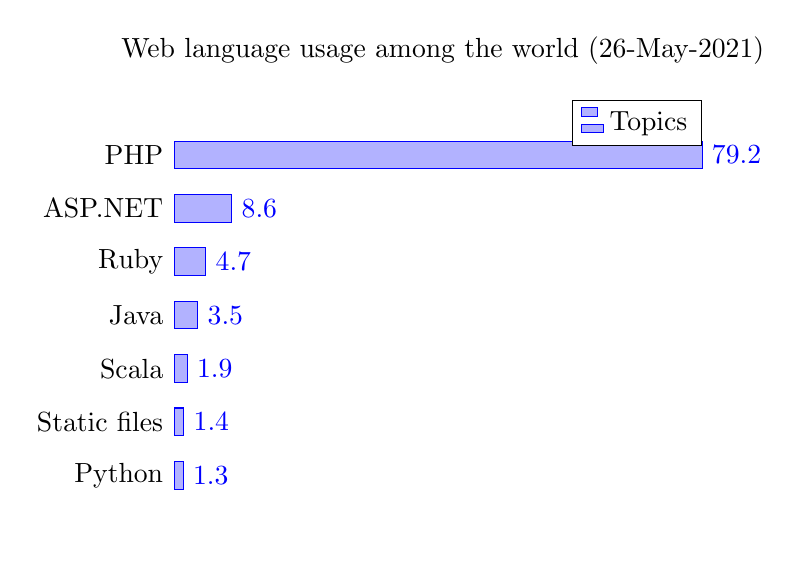
\begin{tikzpicture}
            \begin{axis}[title  = Web language usage among the world (26-May-2021),
                xbar,
                y axis line style = { opacity = 0 },
                axis x line       = none,
                tickwidth         = 0pt,
                ytick             = data,
                enlarge y limits  = 0.2,
                enlarge x limits  = 0.02,
                symbolic y coords = {Python, Static files, Scala, Java, Ruby, ASP.NET,  PHP},
                nodes near coords,
            ]
                \addplot coordinates { (79.2,PHP)         (8.6,ASP.NET)
                (4.7,Ruby)  (3.5,Java) (1.9,Scala) (1.4,Static files) (1.3,Python) };
                \legend{Topics, Posts}
            \end{axis}
        \end{tikzpicture}

        \url{https://w3techs.com/technologies/overview/programming_language}



    \newpage
%    Project structure
%    \subsection{Project structure}\label{subsec:ProjectStructure}

    This is the docker network distribution:
    \begin{center}
    \includegraphics[scale=1]{NetworkDistribution}
    \end{center}


\end{document}